\section{DEMUCS}
D{\'{e}}fossez et al. \cite{defossez2020} proposed a real-time causal speech enhancement model that operates directly on raw waveforms. The authors adopted an encoder-decoder architecture with skip-connections. This model, which has been optimized across time and frequency domains using several loss functions, has been empirically shown to be effective at eliminating a wide range of background noises, including both stationary and non-stationary forms, as well as room reverb. Evaluations using common benchmarks, which include objective metrics and human judgements, show that the model achieves cutting-edge performance for both causal and non-causal approaches while operating directly on the raw waveform.

Inspired by recent improvements, the authors suggest a real-time adaption of the DEMUCS \cite{demucs} architecture for speech enhancement. This architecture uses a causal model based on convolutions and LSTMs, with a frame size of 40ms and a stride of 16ms, and executes faster than real-time on a single laptop processor core. To improve audio quality, the model uses hierarchical generation (similar to U-Net\cite{ronneberger2015u-net} skip-connections) to transition from waveform to waveform.

\subsection{Model Architecture}
DEMUCS consists in a multi-layer convolutional encoder and decoder with U-net \cite{ronneberger2015u-net} skip connections, and a sequence modeling network applied on the encoders' output. It is characterized by its number of layers $L$, initial number of hidden channels $H$, layer kernel size $K$ and stride $S$ and resampling factor $U$. The encoder and decoder layers are numbered from $1$ to $L$ (in reverse order for the decoder, so layers at the same scale have the same index). As the main focus is  on monophonic speech enhancement, the input and output of the model has a single channel only.

Formally, the encoder network $E$ receives the raw waveform as input and produces a latent representation $E(x) = z$. Each layer consists of a convolution layer with a kernel size of $K$ and stride of S with $2^{i-1}$ $H$ output channels, followed by a ReLU activation, a 1x1 convolution with $2^i$ $H$ output channels, and finally a GLU activation that converts the number of channels back to $2^{i-1}$ $H$ as demonstrated in Figure \ref{fig:demucs-encoder-decoder}.

A sequence modelling $R$ network uses the latent representation $z$ as input and produces a non-linear transformation of the same size, $R(z) = LSTM(z) + z$, denoted as $\hat{z}$. The LSTM network is composed of two layers and $2^{L-1}$ $H$ hidden units. For causal prediction, a unidirectional LSTM is employed, whereas for non-causal models, a bidirectional LSTM is used, followed by a linear layer that combines the two outputs.

Finally, a decoder network $D$ accepts $\hat{z}$ as input and returns an estimated clean signal $D(\hat{z}) = \hat{y}$. The i-th layer of the decoder takes as input $2^{i-1}$ $H$ channels and applies a 1x1 convolution with $2^i$ $H$ channels, followed by a GLU activation function that outputs $2^{i-1}$ $H$ channels and finally a transposed convolution with a kernel size of $8$, stride of $4$, and $2^{i-2}$ $H$ output channels, accompanied by a ReLU function. For the last layer, the output is a single channel with no ReLU. As shown in Figure \ref{fig:demucs-arch}, a skip connection connects the encoder's i-th layer output to the decoder's i-th layer input.

\begin{figure}
    \centering
    \begin{minipage}{.5\textwidth}
        \centering
        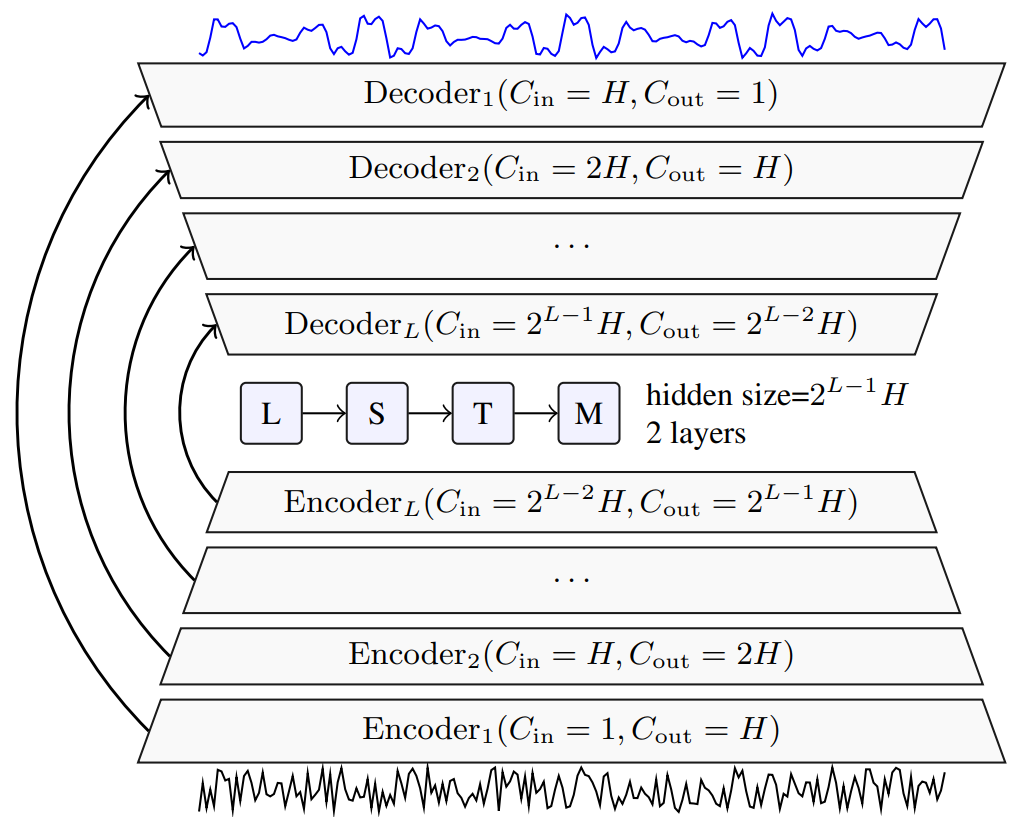
\includegraphics[width=0.9\linewidth]{images/related_work/demucs/demucs-arch.png}
        \caption{Causal DEMUCS with the noisy speech as input on the bottom and the clean speech as output on the top. Arrows represent U-Net skip connections. $H$ controls the number of channels in the model and $L$ its depth.}
        \label{fig:demucs-arch}
    \end{minipage}%
    \begin{minipage}{.5\textwidth}
        \centering
        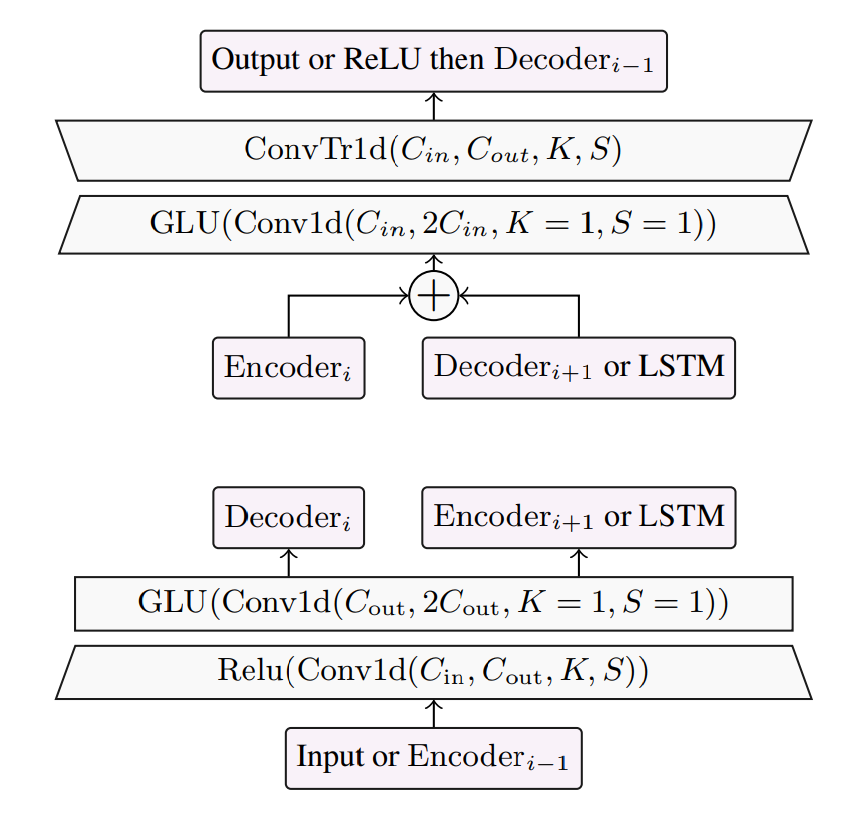
\includegraphics[width=0.8\linewidth]{images/related_work/demucs/demucs-encoder-decoder.png}
        \caption{View of each encoder (bottom) and decoder layer (top). Arrows are connections to other parts of the model. $C_{in}$ (resp. $C_{out}$) is the number of input channels (resp. output), $K$ the kernel size and $S$ the stride.}
        \label{fig:demucs-encoder-decoder}
    \end{minipage}
\end{figure}

\subsection{Experimental Setup}

\subsubsection{Dataset}
The authors used a synthesized subset of DNS 2020 dataset \cite{reddy2020} and Valentini \cite{valentini2016} dataset. They also applied several augmentation techniques:
\begin{itemize}
    \item \textbf{Random Shift:} randomly shifts the signal in time.
    \item \textbf{RevEcho:} adds decaying echoes to the training data.
    \item \textbf{Remix:} shuffles noises within a local batch to form new noisy mixtures.
    \item \textbf{BandMask:} removes 20\% of frequencies uniformly at mel scale.
\end{itemize}
Random shift was applied to all datasets, Remix and BandMask were applied to Valentini \cite{valentini2016}, and RevEcho was applied to DNS \cite{reddy2020}.

\subsubsection{Training}
The authors trained the DEMUCS model for 400 epochs on the Valentini \cite{valentini2016} dataset and 250 on the DNS \cite{reddy2020} dataset. They used the L1 loss between the predicted and ground truth clean speech waveforms, and for the Valentini dataset, also added the STFT loss, which is defined as the sum of the \textit{spectral convergence (sc)} loss and the \textit{magnitude (mag)} loss as follows:
\begin{equation}
    \begin{split}
        L_{\text{stft}}(y,\hat{y}) = L_{\text{sc}}(y,\hat{y}) + L_{\text{mag}}(y,\hat{y})\\
        L_{\text{sc}}(y,\hat{y}) = \frac{\lVert |STFT(y)| - |STFT(\hat{y})| \rVert _{F}}{\lVert |STFT(y)| \rVert _{F}}\\
        L_{\text{mag}}(y,\hat{y}) = \frac{1}{T} \lVert \log{|STFT(y)|} - \log{|STFT(\hat{y})|} \rVert _{1}
    \end{split}
\end{equation}
where $y$ and $\hat{y}$ are the clean signal and the enhanced signal respectively, $\lVert \cdot \rVert _F$ and $\lVert \cdot \rVert _1$ are the Frobenius and $L_1$ norms respectively. The STFT loss was added with a weight of $0.5$. They used the Adam optimizer with a step size of $3e^{-4}$, a momentum of $\beta_1$ = $0.9$ and a denominator momentum $\beta_2$ = $0.999$. For the Valentini dataset, the authors used the original validation set and kept the best model, for the DNS dataset they trained without a validation set and kept the last model. The audio is sampled at $16$ kHz.

\subsection{Conclusion}
The paper presents a novel causal speech enhancement model that operates in the raw waveform domain and runs in real-time on a laptop CPU. The model is capable of removing various types of background noise and has been optimized for both time and frequency domains. The proposed model also includes data augmentation techniques to further improve its performance and generalization abilities. Evaluations on standard benchmarks show that the proposed model matches state-of-the-art performance of both causal and non-causal methods while working directly on the raw waveform. The model is also found to be beneficial for improving an ASR model under noisy conditions. Overall, the proposed model presents a promising solution for real-time speech enhancement in various applications.